\label{key}\documentclass[letterpaper, 12pt,oneside]{article}
\usepackage{amsmath}
\usepackage{graphicx}
\usepackage{xcolor}
\graphicspath{{Imagenes/}}
\usepackage[utf8]{inputenc}
\usepackage{listings}
\usepackage[hidelinks]{hyperref}

\title{\Huge Taller de Herramientas Computacionales}
\author{Josué Artemio Hernández Rodríguez}
\date{24/Enero/2019}

\begin{document}
	\maketitle
	\begin{center}
		
\includegraphics[scale=0.7]{3.jpg}
	\end{center}

	\newpage
	
	\title{\huge \textit{Bitácora problema 6 }}\\

	Este problema te pide 10 números, y de esos números te calcula su promedio. Fue sencillo que implementar una función prom(a,b,c,d,e,f,g,h,i,j): porque depende de esos 10 valores, y en el bucle los cálculos de la suma de esos números y después la división por el numero de valores, es decir 10. Y la solución, que me pidiera los números con un solo imput con los valores separados con comas. 
	 

	\begin{figure}[h]
		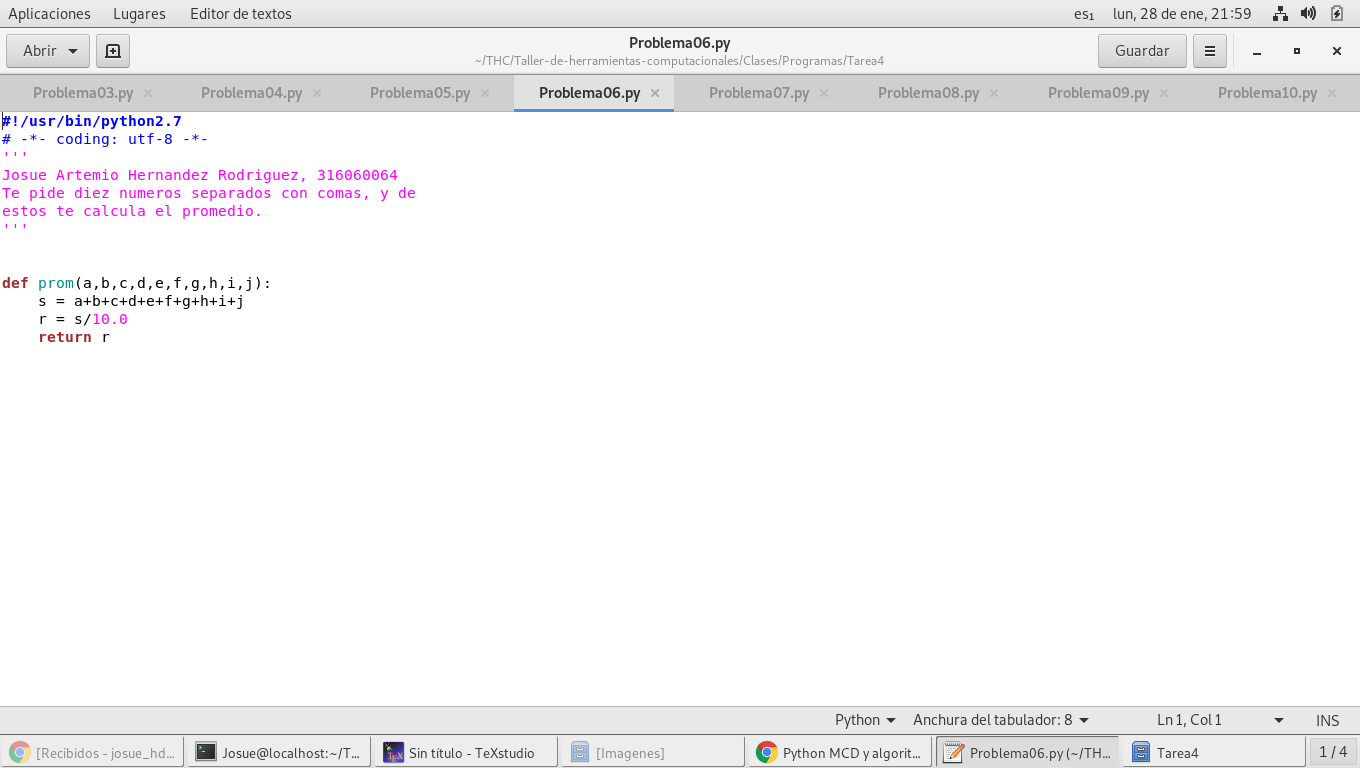
\includegraphics[scale=0.3]{pro06.png}
	\end{figure}
	
	
	
	
	
	
	
	
	
	
	
\end{document}
